\section{Experimentales Setup}
Server mit 4 Graka:

2 mal Geforce GTX 1080 Ti mit CUDA Version 10.1 


2 mal Geforce RTX 2080 Ti mit CUDA Version 10.1

\subsection{Wahl des Frameworks}

Es wird mit pytorch gearbeitet, da pytorch gegenüber anderen Frameworks eine grössere Flexibiltät erlaubt. Ausserdem ist eine fast vollständige, gute Implementierung von PruneTrain in Pytorch geschrieben. Diese wird im nächsten Kapitel untersucht und soweit erweitert, dass es dem Stand im PruneTrain Paper entspricht.



\section{Untersuchung von PruneTrain}

\subsection{Aufbau des CNNs}
Die PruneTrain Implementierung hat initial mehrere verschiedene Netzarchitekturen zur Auswahl:
\begin{itemize}
 \item AlexNet
 \item ResNet 32/50
 \item vgg 8/11/13/16
 \item mobilenet
\end{itemize}

Schränke diese Auswahl auf ResNet ein.
Gründe hierfür:
\begin{itemize}
 \item Da die Überlegung besteht diese Netze tiefer zu machen wähle ResNet, da die Identity-Übergänge dem Netz erlauben das degradation Problem zu umgehen während das Netz noch tiefer/ breiter wird.
 \item Festlegung auf eine Architektur um Umfang der Arbeit zu begrenzen
\end{itemize}




Erweitere dies jedoch durch beliebige grosse ResNets. Ein ResNet ist hier durch 3 grössen charaterisiert:



\begin{itemize}
 \item $s$: Anzahl an Stages, die dasResNet hat
 \item $n:$ Anzahl von Blöcken pro Stage 
 \item $l$: Anzahl von (Conv+Batch)-Layer pro Block
\end{itemize}
$$\text{ResNet-Zahl}=s\cdot n \cdot l$$


\subsection{Einfluss der Batch Größe}
Im PruneTrain paper ist angegeben, dass die Batch Size so gross gewählt wird, dass der GPU Speicher komplett ausgenutzt wird. Dies ist in der vorliegenden Implementierung noch nicht geschehen. Ein direktes Auslesen des allokierbaren Speichers ist relativ schwer zu realisieren mit pytorch. Daher wird ein Modell zur Bestimmung der maximalen Batch Size gebildet.

Hierfür wird für einige verschiedene Modellgrößen durch eine binäre Suche die maximale Batch Size ermittelt. Gleichzeitig wird für die jewilige Modellgrösse die Anzahl an Parametern, die das Modell hat gezählt.
\todo[inline]{Tabelle}

Mit Hilfe dieser Grössen wird für jede einzelne Stagegröße eine Gerade gefittet.

\todo[inline]{Wie gut fittet die Geraden die gegebenen Punkte}
\todo[inline,color=brown]{Überprüfe, ob dies auch bei einem anderen Datensatz funktioniert. Es sollte funktionieren, wenn die Grösse eines anderen Datensatzes ins Verhältnis zu der Grösse in Cifar10 gesetzt wird}


Es stellt sich die Frage, ob das einen so grossen Einfluss auf die Ausführungszeit hat.

\begin{figure}[h]
 \centering
 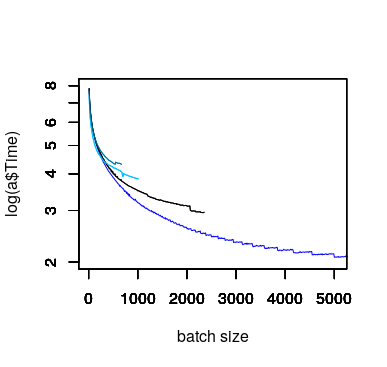
\includegraphics[width=0.8\textwidth]{KapitelPartB/Images/batchSizevsTime.png}
 % batchSizevsTime.png: 387x367 px, 96dpi, 10.24x9.71 cm, bb=0 0 290 275
 \caption{Batch Size vs Trainings Time über eine Epoche}
 \label{fig:batchVsTime}
\end{figure}


Man sieht, dass mit steigender Batchgröße die Ausführungszeit sinkt. 

Errechne zusätzlich noch ein Modell, wo abhängig von der Modellgrösse währenddem Pruning die Batchgrösse angepasst wird.



\cite{largeBatch} gibt an, dass mit grösserer Batch size die Accuracy weniger wird. Aber dort wird ein Verfahren angegben, welches diesen Effekt entfernen kann.
Da dieser Effekt da sehr deutlich gezeigt wird hier im nächsten Unterkapitel nur die Überprüfung, ob dieser Effekt auf bei geprunten Netzwerken funktioniert.
\subsection{Einfluss der Batchgrösse und der Lernrate auf die Verkleinerung des Netzes}
\todo[inline,color=blue]{Untersuche, ob largeBatch auch auf ein PruneTrain Netzwerk anwendbar ist.}
\todo[inline,color=brown]{Untersuche, ob die Grösse des Batches beeinflusst, wie viel vom Netz geprunt wird}


\subsection{Nachvollziehbarkeit der PruneTrain Ergebnisse}
\todo[inline]{Nachvollziehen der PruneTrain Ergebnisse mit dieser Implementierung}

\section{PruneTrain als MorphNet}

\subsection{Net 2 Net}
\todo[inline]{Zeige wie Net2Net aus einem Netzwerk ein tieferes oder breiteres Netz macht}

\subsection{Morphnet}
MorphNet macht alle Layer breiter um sie dann mit einem speziellen Regularisierer breiter zu machen. Dieser Regularisierer hat verschiedene mögliche Zielgrössen (Modelgrösse, Flops oder Inferenz-Zeit).
Die Frage stellt sich hier, ob das Netz besser wird wenn alle Schichten breiter gemacht werden um später wieder geprunt zuwerden.
\todo[inline,color=blue]{Vollziehe mit PrunTrain + Net2Net nach, ob dies funktioniert wie MorphNet}

Weiterhin besteht die Möglichkeit das Netz nicht nur breiter zu machen sondern auch tiefer.
\todo[inline,color=brown]{Mache das Netz tiefer}
\todo[inline, color =blue]{Suche Kriterien, die entscheiden ob das Netz tiefer sein sollte}


MorphNet erwähnt, dass es Sinn macht nicht im ganzen Netz denn Wider Operator anzuwenden sonder nur da wo der Regularisierer das Netz nicht schmaller macht.
\todo[inline, color=blue]{Entwickle Möglichkeit dies direkter da anzuwenden, wo nicht geprunt wurde}


\section{Überblick über die möglichen Strategien}

Welche Strategien aus Kapitel 2 sind überhaupt durchführbar?
Hier werden nur die Strategien aufgeführt, welche überhaupt auf vernünftig grossen Datensätzen funktionieren und von der Technik und dem Aufwand her möglich sind.
Die Strategien sind aufgeteilt in Unterkapitel. 

Alle möglichen Kombinationen von Strategien sind zuviele. Daher sinnvolle Vorauswahl treffen.  
Bei mehreren gleichartigen/ konkurierenden Ansätze drekter Vergleich und dann den besten auswählen.
\subsection{Zahlenformate}

\begin{itemize}
 \item FP16 bereits probiert
\end{itemize}


FP16 nur auf RTX 2080 sinnvoll
Bietet nach erster Messung etwa 28 \% Prozent Gewinn.

Code für dieses Verfahren liegt vor: Amp apex von Nvidia

AMP bietet 3 mögliche Optimierungsstufen:

O1
Patch all Torch functions and Tensor methods to cast their inputs according to a whitelist-blacklist model. Whitelist ops (for example, Tensor Core-friendly ops like GEMMs and convolutions) are performed in FP16. Blacklist ops that benefit from FP32 precision (for example, softmax) are performed in FP32. O1 also uses dynamic loss scaling, unless overridden.

02
casts the model weights to FP16, patches the models forward method to cast input data to FP16, keeps batchnorms in FP32, maintains FP32 master weights, updates the optimizer’s paramgroups so that the optimizer.step() acts directly on the FP32 weights (followed by FP32 master weight-FP16 model weight copies if necessary), and implements dynamic loss scaling (unless overridden). Unlike O1, O2 does not patch Torch functions or Tensor methods.


O3
may not achieve the stability of the true mixed precision options O1 and O2. However, it can be useful to establish a speed baseline for your model, against which the performance of O1 and O2 can be compared. If your model uses batch normalization, to establish speed of light you can try O3 with the additional property override keepBatchnormfp32=True (which enables cudnn batchnorm, as stated earlier).

Hier nur O0, O1 und O2 dargestellt, da O3 absolut nicht mithalten kann was Performance angeht.

\begin{figure}[h]
 \centering
 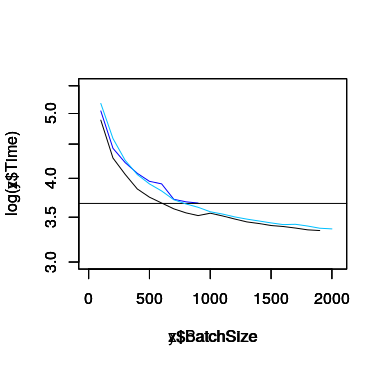
\includegraphics[width=0.8\textwidth]{KapitelPartB/Images/timeVsBatchSize_Amp.png}
 % timeVsBatchSize_Amp.png: 387x367 px, 96dpi, 10.24x9.71 cm, bb=0 0 290 275
 \caption{Vergleich Trainingszeit einer Epoche für verschiedene Optimierungsstufen von Amp Apex. DunkelBlau=O0; Schwarz = O1; Hellblau=O2}
 \label{fig:amp}
\end{figure}

\todo[inline,color=brown]{Weitere Versuche, die zeigen ob die Zeiten grossen statistischen Schwankungen unterliegen.}
\url{https://developer.download.nvidia.com/video/gputechconf/gtc/2019/presentation/s9998-automatic-mixed-precision-in-pytorch.pdf} zeigt, dass bezüglich der Accuracy kein Verlust zu erwarten ist.

Da O2 gegenüber O1 keinen signifikanten zusätzlichen Gewinn bringt nutze O1.
\subsection{Beschleunigung der Berechnung des Gradientenabstiegverfahren}


Accelerating CNN Training by Sparsifying Activation Gradients funktioniert nur auf Toy-Benchmarks 


\subsubsection{Weight Normalization: A Simple Reparameterization
to Accelerate Training of Deep Neural Networks}

\todo[inline,color=blue]{Testen ob es funktioniert}
Könnte funktionieren. Code für Lasagne: https://github.com/TimSalimans/weight\_norm


\subsubsection{Accelerating Deep Neural Network Training with Inconsistent Stochastic Gradient Descent}

Interessant bisher kein Code verfügbar
\todo[inline, color=blue]{Implementieren (ist einfach) und testen}

\subsubsection{Accelerated CNN Training Through Gradient Approximation }

Interessant bisher kein Code verfügbar


\subsubsection{Sind diese Verfahren theoretisch kombinierbar}
\todo[inline,color=blue]{Testen, wenn die anderen funktionieren}
\subsection{Verfahren um weniger Trainingsdaten zu verwenden}


\subsubsection{Stochastisches Pooling}

Klingt sehr interessant und könnte für deutlich kleinere Trainingsdatenmenge sorgen
Oder alternativ bei gleicher Trainingsdatenmenge die Accuracy verbessern
https://github.com/Shuangfei/s3pool
\todo[inline,color=blue]{Testen}

\subsection{Lernen von Struktur und Stärke von CNNs}

bisher kein Code verfügbar.Klingt aber interessant
\todo[inline]{Ist zwar interessant aber ohne Code dazu wohl zu aufwändig}




\section{Schnelleres MorphPruneTrain}
FP16 + plus ein Verfahren aus dem Bereich Gradienten

\todo[inline, color=blue]{Funktioniert erst, wenn die anderen Experimente durchgelaufen sind}
